\documentclass[1p]{elsarticle_modified}
%\bibliographystyle{elsarticle-num}

%\usepackage[colorlinks]{hyperref}
%\usepackage{abbrmath_seonhwa} %\Abb, \Ascr, \Acal ,\Abf, \Afrak
\usepackage{amsfonts}
\usepackage{amssymb}
\usepackage{amsmath}
\usepackage{amsthm}
\usepackage{scalefnt}
\usepackage{amsbsy}
\usepackage{kotex}
\usepackage{caption}
\usepackage{subfig}
\usepackage{color}
\usepackage{graphicx}
\usepackage{xcolor} %% white, black, red, green, blue, cyan, magenta, yellow
\usepackage{float}
\usepackage{setspace}
\usepackage{hyperref}

\usepackage{tikz}
\usetikzlibrary{arrows}

\usepackage{multirow}
\usepackage{array} % fixed length table
\usepackage{hhline}

%%%%%%%%%%%%%%%%%%%%%
\makeatletter
\renewcommand*\env@matrix[1][\arraystretch]{%
	\edef\arraystretch{#1}%
	\hskip -\arraycolsep
	\let\@ifnextchar\new@ifnextchar
	\array{*\c@MaxMatrixCols c}}
\makeatother %https://tex.stackexchange.com/questions/14071/how-can-i-increase-the-line-spacing-in-a-matrix
%%%%%%%%%%%%%%%

\usepackage[normalem]{ulem}

\newcommand{\msout}[1]{\ifmmode\text{\sout{\ensuremath{#1}}}\else\sout{#1}\fi}
%SOURCE: \msout is \stkout macro in https://tex.stackexchange.com/questions/20609/strikeout-in-math-mode

\newcommand{\cancel}[1]{
	\ifmmode
	{\color{red}\msout{#1}}
	\else
	{\color{red}\sout{#1}}
	\fi
}

\newcommand{\add}[1]{
	{\color{blue}\uwave{#1}}
}

\newcommand{\replace}[2]{
	\ifmmode
	{\color{red}\msout{#1}}{\color{blue}\uwave{#2}}
	\else
	{\color{red}\sout{#1}}{\color{blue}\uwave{#2}}
	\fi
}

\newcommand{\Sol}{\mathcal{S}} %segment
\newcommand{\D}{D} %diagram
\newcommand{\A}{\mathcal{A}} %arc


%%%%%%%%%%%%%%%%%%%%%%%%%%%%%5 test

\def\sl{\operatorname{\textup{SL}}(2,\Cbb)}
\def\psl{\operatorname{\textup{PSL}}(2,\Cbb)}
\def\quan{\mkern 1mu \triangleright \mkern 1mu}

\theoremstyle{definition}
\newtheorem{thm}{Theorem}[section]
\newtheorem{prop}[thm]{Proposition}
\newtheorem{lem}[thm]{Lemma}
\newtheorem{ques}[thm]{Question}
\newtheorem{cor}[thm]{Corollary}
\newtheorem{defn}[thm]{Definition}
\newtheorem{exam}[thm]{Example}
\newtheorem{rmk}[thm]{Remark}
\newtheorem{alg}[thm]{Algorithm}

\newcommand{\I}{\sqrt{-1}}
\begin{document}

%\begin{frontmatter}
%
%\title{Boundary parabolic representations of knots up to 8 crossings}
%
%%% Group authors per affiliation:
%\author{Yunhi Cho} 
%\address{Department of Mathematics, University of Seoul, Seoul, Korea}
%\ead{yhcho@uos.ac.kr}
%
%
%\author{Seonhwa Kim} %\fnref{s_kim}}
%\address{Center for Geometry and Physics, Institute for Basic Science, Pohang, 37673, Korea}
%\ead{ryeona17@ibs.re.kr}
%
%\author{Hyuk Kim}
%\address{Department of Mathematical Sciences, Seoul National University, Seoul 08826, Korea}
%\ead{hyukkim@snu.ac.kr}
%
%\author{Seokbeom Yoon}
%\address{Department of Mathematical Sciences, Seoul National University, Seoul, 08826,  Korea}
%\ead{sbyoon15@snu.ac.kr}
%
%\begin{abstract}
%We find all boundary parabolic representation of knots up to 8 crossings.
%
%\end{abstract}
%\begin{keyword}
%    \MSC[2010] 57M25 
%\end{keyword}
%
%\end{frontmatter}

%\linenumbers
%\tableofcontents
%
\newcommand\colored[1]{\textcolor{white}{\rule[-0.35ex]{0.8em}{1.4ex}}\kern-0.8em\color{red} #1}%
%\newcommand\colored[1]{\textcolor{white}{ #1}\kern-2.17ex	\textcolor{white}{ #1}\kern-1.81ex	\textcolor{white}{ #1}\kern-2.15ex\color{red}#1	}

{\Large $\underline{9_{41}~(K9a_{29})}$}

\setlength{\tabcolsep}{10pt}
\renewcommand{\arraystretch}{1.6}
\vspace{1cm}\begin{tabular}{m{100pt}>{\centering\arraybackslash}m{274pt}}
\multirow{5}{120pt}{
	\centering
	\includegraphics[width=112pt]{../../../GIT/diagram.site/Diagrams/png/76_9_41.png}\\
\ \ \ A knot diagram\footnotemark}&
\allowdisplaybreaks
\textbf{Linearized knot diagam} \\
\cline{2-2}
 &
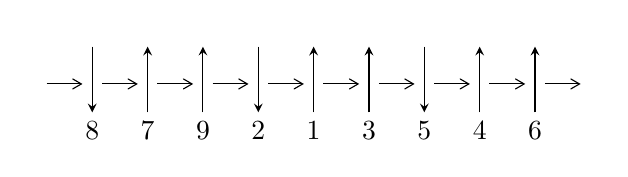
\begin{tikzpicture}[x=20pt, y=17pt]
	% nodes
	\node (C0) at (0, 0) {};
	\node (C1) at (1, 0) {};
	\node (C1U) at (1, +1) {};
	\node (C1D) at (1, -1) {8};

	\node (C2) at (2, 0) {};
	\node (C2U) at (2, +1) {};
	\node (C2D) at (2, -1) {7};

	\node (C3) at (3, 0) {};
	\node (C3U) at (3, +1) {};
	\node (C3D) at (3, -1) {9};

	\node (C4) at (4, 0) {};
	\node (C4U) at (4, +1) {};
	\node (C4D) at (4, -1) {2};

	\node (C5) at (5, 0) {};
	\node (C5U) at (5, +1) {};
	\node (C5D) at (5, -1) {1};

	\node (C6) at (6, 0) {};
	\node (C6U) at (6, +1) {};
	\node (C6D) at (6, -1) {3};

	\node (C7) at (7, 0) {};
	\node (C7U) at (7, +1) {};
	\node (C7D) at (7, -1) {5};

	\node (C8) at (8, 0) {};
	\node (C8U) at (8, +1) {};
	\node (C8D) at (8, -1) {4};

	\node (C9) at (9, 0) {};
	\node (C9U) at (9, +1) {};
	\node (C9D) at (9, -1) {6};
	\node (C10) at (10, 0) {};

	% arrows
	\draw[->,>={angle 60}]
	(C0) edge (C1) (C1) edge (C2) (C2) edge (C3) (C3) edge (C4) (C4) edge (C5) (C5) edge (C6) (C6) edge (C7) (C7) edge (C8) (C8) edge (C9) (C9) edge (C10) ;	\draw[->,>=stealth]
	(C1U) edge (C1D) (C2D) edge (C2U) (C3D) edge (C3U) (C4U) edge (C4D) (C5D) edge (C5U) (C6D) edge (C6U) (C7U) edge (C7D) (C8D) edge (C8U) (C9D) edge (C9U) ;
	\end{tikzpicture} \\
\hhline{~~} \\& 
\textbf{Solving Sequence} \\ \cline{2-2} 
 &
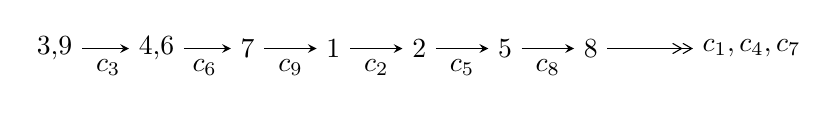
\begin{tikzpicture}[x=31pt, y=7pt]
	% node
	\node (A0) at (-1/8, 0) {3,9};
	\node (A1) at (17/16, 0) {4,6};
	\node (A2) at (17/8, 0) {7};
	\node (A3) at (25/8, 0) {1};
	\node (A4) at (33/8, 0) {2};
	\node (A5) at (41/8, 0) {5};
	\node (A6) at (49/8, 0) {8};
	\node (C1) at (1/2, -1) {$c_{3}$};
	\node (C2) at (13/8, -1) {$c_{6}$};
	\node (C3) at (21/8, -1) {$c_{9}$};
	\node (C4) at (29/8, -1) {$c_{2}$};
	\node (C5) at (37/8, -1) {$c_{5}$};
	\node (C6) at (45/8, -1) {$c_{8}$};
	\node (A7) at (8, 0) {$c_{1},c_{4},c_{7}$};

	% edge
	\draw[->,>=stealth]	
	(A0) edge (A1) (A1) edge (A2) (A2) edge (A3) (A3) edge (A4) (A4) edge (A5) (A5) edge (A6) ;
	\draw[->>,>={angle 60}]	
	(A6) edge (A7);
\end{tikzpicture} \\ 

\end{tabular} \\

\footnotetext{
The image of knot diagram is generated by the software ``\textbf{Draw programme}" developed by Andrew Bartholomew(\url{http://www.layer8.co.uk/maths/draw/index.htm\#Running-draw}), where we modified some parts for our purpose(\url{https://github.com/CATsTAILs/LinksPainter}).
}\phantom \\ \newline 
\centering \textbf{Ideals for irreducible components\footnotemark of $X_{\text{par}}$} 
 
\begin{align*}
I^u_{1}&=\langle 
b+u,\;a-1,\;u^4-2 u^3+4 u^2-3 u+1\rangle \\
I^u_{2}&=\langle 
b+u,\;a^2+a u+2 u^2+2 a+2 u+4,\;u^3+u^2+2 u+1\rangle \\
I^u_{3}&=\langle 
-3 u^5+11 u^4-26 u^3+35 u^2+4 b-28 u+12,\;3 u^5-9 u^4+20 u^3-23 u^2+8 a+14 u-4,\\
\phantom{I^u_{3}}&\phantom{= \langle  }u^6-5 u^5+14 u^4-25 u^3+28 u^2-20 u+8\rangle \\
I^u_{4}&=\langle 
- u^2 b+b^2-2 b u-2 u,\;a-1,\;u^3+u^2+2 u+1\rangle \\
I^u_{5}&=\langle 
b+u,\;a+1,\;u^4+2 u^2- u+1\rangle \\
I^u_{6}&=\langle 
- a u+b- u-1,\;- u^2 a+a^2- a u+3 u^2- a+u+5,\;u^3+u^2+2 u+1\rangle \\
\\
\end{align*}
\raggedright * 6 irreducible components of $\dim_{\mathbb{C}}=0$, with total 32 representations.\\
\footnotetext{All coefficients of polynomials are rational numbers. But the coefficients are sometimes approximated in decimal forms when there is not enough margin.}
\newpage
\renewcommand{\arraystretch}{1}
\centering \section*{I. $I^u_{1}= \langle b+u,\;a-1,\;u^4-2 u^3+4 u^2-3 u+1 \rangle$}
\flushleft \textbf{(i) Arc colorings}\\
\begin{tabular}{m{7pt} m{180pt} m{7pt} m{180pt} }
\flushright $a_{3}=$&$\begin{pmatrix}1\\0\end{pmatrix}$ \\
\flushright $a_{9}=$&$\begin{pmatrix}0\\u\end{pmatrix}$ \\
\flushright $a_{4}=$&$\begin{pmatrix}1\\- u^2\end{pmatrix}$ \\
\flushright $a_{6}=$&$\begin{pmatrix}1\\- u\end{pmatrix}$ \\
\flushright $a_{7}=$&$\begin{pmatrix}- u+1\\- u\end{pmatrix}$ \\
\flushright $a_{1}=$&$\begin{pmatrix}u\\- u^2+u\end{pmatrix}$ \\
\flushright $a_{2}=$&$\begin{pmatrix}u^2- u+1\\u^2\end{pmatrix}$ \\
\flushright $a_{5}=$&$\begin{pmatrix}u^2+1\\- u^3+u^2- u\end{pmatrix}$ \\
\flushright $a_{8}=$&$\begin{pmatrix}- u\\u^3+u\end{pmatrix}$\\ \flushright $a_{8}=$&$\begin{pmatrix}- u\\u^3+u\end{pmatrix}$\\&\end{tabular}
\flushleft \textbf{(ii) Obstruction class $= -1$}\\~\\
\flushleft \textbf{(iii) Cusp Shapes $= -3 u^3+9 u^2-18 u+15$}\\~\\
\newpage\renewcommand{\arraystretch}{1}
\flushleft \textbf{(iv) u-Polynomials at the component}\newline \\
\begin{tabular}{m{50pt}|m{274pt}}
Crossings & \hspace{64pt}u-Polynomials at each crossing \\
\hline $$\begin{aligned}c_{1},c_{4},c_{7}\end{aligned}$$&$\begin{aligned}
&u^4-3 u^3+4 u^2-2 u+1
\end{aligned}$\\
\hline $$\begin{aligned}c_{2},c_{3},c_{5}\\c_{6},c_{8},c_{9}\end{aligned}$$&$\begin{aligned}
&u^4-2 u^3+4 u^2-3 u+1
\end{aligned}$\\
\hline
\end{tabular}\\~\\
\newpage\renewcommand{\arraystretch}{1}
\flushleft \textbf{(v) Riley Polynomials at the component}\newline \\
\begin{tabular}{m{50pt}|m{274pt}}
Crossings & \hspace{64pt}Riley Polynomials at each crossing \\
\hline $$\begin{aligned}c_{1},c_{4},c_{7}\end{aligned}$$&$\begin{aligned}
&y^4- y^3+6 y^2+4 y+1
\end{aligned}$\\
\hline $$\begin{aligned}c_{2},c_{3},c_{5}\\c_{6},c_{8},c_{9}\end{aligned}$$&$\begin{aligned}
&y^4+4 y^3+6 y^2- y+1
\end{aligned}$\\
\hline
\end{tabular}\\~\\
\newpage\flushleft \textbf{(vi) Complex Volumes and Cusp Shapes}
$$\begin{array}{c|c|c}  
\text{Solutions to }I^u_{1}& \I (\text{vol} + \sqrt{-1}CS) & \text{Cusp shape}\\
 \hline 
\begin{aligned}
u &= \phantom{-}0.500000 + 0.363271 I \\
a &= \phantom{-}1.00000\phantom{ +0.000000I} \\
b &= -0.500000 - 0.363271 I\end{aligned}
 & \phantom{-}0.986960 + 0.735995 I & \phantom{-}7.28115 - 3.94298 I \\ \hline\begin{aligned}
u &= \phantom{-}0.500000 - 0.363271 I \\
a &= \phantom{-}1.00000\phantom{ +0.000000I} \\
b &= -0.500000 + 0.363271 I\end{aligned}
 & \phantom{-}0.986960 - 0.735995 I & \phantom{-}7.28115 + 3.94298 I \\ \hline\begin{aligned}
u &= \phantom{-}0.50000 + 1.53884 I \\
a &= \phantom{-}1.00000\phantom{ +0.000000I} \\
b &= -0.50000 - 1.53884 I\end{aligned}
 & -10.8566 + 12.0989 I & -2.78115 - 6.37988 I \\ \hline\begin{aligned}
u &= \phantom{-}0.50000 - 1.53884 I \\
a &= \phantom{-}1.00000\phantom{ +0.000000I} \\
b &= -0.50000 + 1.53884 I\end{aligned}
 & -10.8566 - 12.0989 I & -2.78115 + 6.37988 I\\
 \hline 
 \end{array}$$\newpage\newpage\renewcommand{\arraystretch}{1}
\centering \section*{II. $I^u_{2}= \langle b+u,\;a^2+a u+2 u^2+2 a+2 u+4,\;u^3+u^2+2 u+1 \rangle$}
\flushleft \textbf{(i) Arc colorings}\\
\begin{tabular}{m{7pt} m{180pt} m{7pt} m{180pt} }
\flushright $a_{3}=$&$\begin{pmatrix}1\\0\end{pmatrix}$ \\
\flushright $a_{9}=$&$\begin{pmatrix}0\\u\end{pmatrix}$ \\
\flushright $a_{4}=$&$\begin{pmatrix}1\\- u^2\end{pmatrix}$ \\
\flushright $a_{6}=$&$\begin{pmatrix}a\\- u\end{pmatrix}$ \\
\flushright $a_{7}=$&$\begin{pmatrix}a- u\\- u\end{pmatrix}$ \\
\flushright $a_{1}=$&$\begin{pmatrix}- u^2 a-2 a u+2\\- u^2 a+u\end{pmatrix}$ \\
\flushright $a_{2}=$&$\begin{pmatrix}- a u+u^2+1\\u^2\end{pmatrix}$ \\
\flushright $a_{5}=$&$\begin{pmatrix}- u^2 a-5 a u-2 u^2-2 a-4 u\\-2 u^2 a-3 a u-2 u^2- a- u\end{pmatrix}$ \\
\flushright $a_{8}=$&$\begin{pmatrix}- u\\- u^2- u-1\end{pmatrix}$\\ \flushright $a_{8}=$&$\begin{pmatrix}- u\\- u^2- u-1\end{pmatrix}$\\&\end{tabular}
\flushleft \textbf{(ii) Obstruction class $= -1$}\\~\\
\flushleft \textbf{(iii) Cusp Shapes $= 4 a u+8 u^2+4 a+12 u+10$}\\~\\
\newpage\renewcommand{\arraystretch}{1}
\flushleft \textbf{(iv) u-Polynomials at the component}\newline \\
\begin{tabular}{m{50pt}|m{274pt}}
Crossings & \hspace{64pt}u-Polynomials at each crossing \\
\hline $$\begin{aligned}c_{1},c_{7}\end{aligned}$$&$\begin{aligned}
&(u^3+u^2-1)^2
\end{aligned}$\\
\hline $$\begin{aligned}c_{2},c_{3},c_{6}\\c_{8}\end{aligned}$$&$\begin{aligned}
&(u^3+u^2+2 u+1)^2
\end{aligned}$\\
\hline $$\begin{aligned}c_{4}\end{aligned}$$&$\begin{aligned}
&u^6-7 u^5+24 u^4-47 u^3+54 u^2-32 u+8
\end{aligned}$\\
\hline $$\begin{aligned}c_{5},c_{9}\end{aligned}$$&$\begin{aligned}
&u^6-5 u^5+14 u^4-25 u^3+28 u^2-20 u+8
\end{aligned}$\\
\hline
\end{tabular}\\~\\
\newpage\renewcommand{\arraystretch}{1}
\flushleft \textbf{(v) Riley Polynomials at the component}\newline \\
\begin{tabular}{m{50pt}|m{274pt}}
Crossings & \hspace{64pt}Riley Polynomials at each crossing \\
\hline $$\begin{aligned}c_{1},c_{7}\end{aligned}$$&$\begin{aligned}
&(y^3- y^2+2 y-1)^2
\end{aligned}$\\
\hline $$\begin{aligned}c_{2},c_{3},c_{6}\\c_{8}\end{aligned}$$&$\begin{aligned}
&(y^3+3 y^2+2 y-1)^2
\end{aligned}$\\
\hline $$\begin{aligned}c_{4}\end{aligned}$$&$\begin{aligned}
&y^6- y^5+26 y^4-49 y^3+292 y^2-160 y+64
\end{aligned}$\\
\hline $$\begin{aligned}c_{5},c_{9}\end{aligned}$$&$\begin{aligned}
&y^6+3 y^5+2 y^4-25 y^3+8 y^2+48 y+64
\end{aligned}$\\
\hline
\end{tabular}\\~\\
\newpage\flushleft \textbf{(vi) Complex Volumes and Cusp Shapes}
$$\begin{array}{c|c|c}  
\text{Solutions to }I^u_{2}& \I (\text{vol} + \sqrt{-1}CS) & \text{Cusp shape}\\
 \hline 
\begin{aligned}
u &= -0.215080 + 1.307140 I \\
a &= -0.407481 - 0.986732 I \\
b &= \phantom{-}0.215080 - 1.307140 I\end{aligned}
 & -4.93480 - 5.65624 I & -2.00000 + 5.95889 I \\ \hline\begin{aligned}
u &= -0.215080 + 1.307140 I \\
a &= -1.37744 - 0.32041 I \\
b &= \phantom{-}0.215080 - 1.307140 I\end{aligned}
 & -9.07239 - 2.82812 I & -8.52927 + 2.97945 I \\ \hline\begin{aligned}
u &= -0.215080 - 1.307140 I \\
a &= -0.407481 + 0.986732 I \\
b &= \phantom{-}0.215080 + 1.307140 I\end{aligned}
 & -4.93480 + 5.65624 I & -2.00000 - 5.95889 I \\ \hline\begin{aligned}
u &= -0.215080 - 1.307140 I \\
a &= -1.37744 + 0.32041 I \\
b &= \phantom{-}0.215080 + 1.307140 I\end{aligned}
 & -9.07239 + 2.82812 I & -8.52927 - 2.97945 I \\ \hline\begin{aligned}
u &= -0.569840\phantom{ +0.000000I} \\
a &= -0.71508 + 1.73159 I \\
b &= \phantom{-}0.569840\phantom{ +0.000000I}\end{aligned}
 & -0.79722 - 2.82812 I & \phantom{-}4.52927 + 2.97945 I \\ \hline\begin{aligned}
u &= -0.569840\phantom{ +0.000000I} \\
a &= -0.71508 - 1.73159 I \\
b &= \phantom{-}0.569840\phantom{ +0.000000I}\end{aligned}
 & -0.79722 + 2.82812 I & \phantom{-}4.52927 - 2.97945 I\\
 \hline 
 \end{array}$$\newpage\newpage\renewcommand{\arraystretch}{1}
\centering \section*{III. $I^u_{3}= \langle -3 u^5+11 u^4+\cdots+4 b+12,\;3 u^5-9 u^4+20 u^3-23 u^2+8 a+14 u-4,\;u^6-5 u^5+14 u^4-25 u^3+28 u^2-20 u+8 \rangle$}
\flushleft \textbf{(i) Arc colorings}\\
\begin{tabular}{m{7pt} m{180pt} m{7pt} m{180pt} }
\flushright $a_{3}=$&$\begin{pmatrix}1\\0\end{pmatrix}$ \\
\flushright $a_{9}=$&$\begin{pmatrix}0\\u\end{pmatrix}$ \\
\flushright $a_{4}=$&$\begin{pmatrix}1\\- u^2\end{pmatrix}$ \\
\flushright $a_{6}=$&$\begin{pmatrix}-\frac{3}{8} u^5+\frac{9}{8} u^4+\cdots-\frac{7}{4} u+\frac{1}{2}\\\frac{3}{4} u^5-\frac{11}{4} u^4+\cdots+7 u-3\end{pmatrix}$ \\
\flushright $a_{7}=$&$\begin{pmatrix}\frac{3}{8} u^5-\frac{13}{8} u^4+\cdots+\frac{21}{4} u-\frac{5}{2}\\\frac{3}{4} u^5-\frac{11}{4} u^4+\cdots+7 u-3\end{pmatrix}$ \\
\flushright $a_{1}=$&$\begin{pmatrix}\frac{5}{8} u^5-\frac{19}{8} u^4+\cdots+\frac{23}{4} u-3\\-\frac{3}{4} u^5+\frac{13}{4} u^4+\cdots-\frac{17}{2} u+5\end{pmatrix}$ \\
\flushright $a_{2}=$&$\begin{pmatrix}\frac{1}{8} u^5-\frac{7}{8} u^4+\cdots+\frac{15}{4} u-1\\\frac{3}{4} u^5-\frac{13}{4} u^4+\cdots+\frac{19}{2} u-5\end{pmatrix}$ \\
\flushright $a_{5}=$&$\begin{pmatrix}-\frac{1}{8} u^5+\frac{5}{8} u^4+\cdots+\frac{13}{8} u^2-\frac{1}{2} u\\- u^5+\frac{7}{2} u^4-\frac{17}{2} u^3+11 u^2-\frac{19}{2} u+5\end{pmatrix}$ \\
\flushright $a_{8}=$&$\begin{pmatrix}- u\\u^3+u\end{pmatrix}$\\ \flushright $a_{8}=$&$\begin{pmatrix}- u\\u^3+u\end{pmatrix}$\\&\end{tabular}
\flushleft \textbf{(ii) Obstruction class $= -1$}\\~\\
\flushleft \textbf{(iii) Cusp Shapes $= - u^5+u^4-2 u^3+u^2-4 u+6$}\\~\\
\newpage\renewcommand{\arraystretch}{1}
\flushleft \textbf{(iv) u-Polynomials at the component}\newline \\
\begin{tabular}{m{50pt}|m{274pt}}
Crossings & \hspace{64pt}u-Polynomials at each crossing \\
\hline $$\begin{aligned}c_{1},c_{4}\end{aligned}$$&$\begin{aligned}
&(u^3+u^2-1)^2
\end{aligned}$\\
\hline $$\begin{aligned}c_{2},c_{5},c_{6}\\c_{9}\end{aligned}$$&$\begin{aligned}
&(u^3+u^2+2 u+1)^2
\end{aligned}$\\
\hline $$\begin{aligned}c_{3},c_{8}\end{aligned}$$&$\begin{aligned}
&u^6-5 u^5+14 u^4-25 u^3+28 u^2-20 u+8
\end{aligned}$\\
\hline $$\begin{aligned}c_{7}\end{aligned}$$&$\begin{aligned}
&u^6-7 u^5+24 u^4-47 u^3+54 u^2-32 u+8
\end{aligned}$\\
\hline
\end{tabular}\\~\\
\newpage\renewcommand{\arraystretch}{1}
\flushleft \textbf{(v) Riley Polynomials at the component}\newline \\
\begin{tabular}{m{50pt}|m{274pt}}
Crossings & \hspace{64pt}Riley Polynomials at each crossing \\
\hline $$\begin{aligned}c_{1},c_{4}\end{aligned}$$&$\begin{aligned}
&(y^3- y^2+2 y-1)^2
\end{aligned}$\\
\hline $$\begin{aligned}c_{2},c_{5},c_{6}\\c_{9}\end{aligned}$$&$\begin{aligned}
&(y^3+3 y^2+2 y-1)^2
\end{aligned}$\\
\hline $$\begin{aligned}c_{3},c_{8}\end{aligned}$$&$\begin{aligned}
&y^6+3 y^5+2 y^4-25 y^3+8 y^2+48 y+64
\end{aligned}$\\
\hline $$\begin{aligned}c_{7}\end{aligned}$$&$\begin{aligned}
&y^6- y^5+26 y^4-49 y^3+292 y^2-160 y+64
\end{aligned}$\\
\hline
\end{tabular}\\~\\
\newpage\flushleft \textbf{(vi) Complex Volumes and Cusp Shapes}
$$\begin{array}{c|c|c}  
\text{Solutions to }I^u_{3}& \I (\text{vol} + \sqrt{-1}CS) & \text{Cusp shape}\\
 \hline 
\begin{aligned}
u &= \phantom{-}0.407481 + 0.986732 I \\
a &= -0.203741 + 0.493366 I \\
b &= \phantom{-}0.569840\phantom{ +0.000000I}\end{aligned}
 & -0.79722 + 2.82812 I & \phantom{-}4.52927 - 2.97945 I \\ \hline\begin{aligned}
u &= \phantom{-}0.407481 - 0.986732 I \\
a &= -0.203741 - 0.493366 I \\
b &= \phantom{-}0.569840\phantom{ +0.000000I}\end{aligned}
 & -0.79722 - 2.82812 I & \phantom{-}4.52927 + 2.97945 I \\ \hline\begin{aligned}
u &= \phantom{-}1.37744 + 0.32041 I \\
a &= -0.357540 - 0.865797 I \\
b &= \phantom{-}0.215080 + 1.307140 I\end{aligned}
 & -4.93480 + 5.65624 I & -2.00000 - 5.95889 I \\ \hline\begin{aligned}
u &= \phantom{-}1.37744 - 0.32041 I \\
a &= -0.357540 + 0.865797 I \\
b &= \phantom{-}0.215080 - 1.307140 I\end{aligned}
 & -4.93480 - 5.65624 I & -2.00000 + 5.95889 I \\ \hline\begin{aligned}
u &= \phantom{-}0.71508 + 1.73159 I \\
a &= -0.688719 - 0.160205 I \\
b &= \phantom{-}0.215080 + 1.307140 I\end{aligned}
 & -9.07239 + 2.82812 I & -8.52927 - 2.97945 I \\ \hline\begin{aligned}
u &= \phantom{-}0.71508 - 1.73159 I \\
a &= -0.688719 + 0.160205 I \\
b &= \phantom{-}0.215080 - 1.307140 I\end{aligned}
 & -9.07239 - 2.82812 I & -8.52927 + 2.97945 I\\
 \hline 
 \end{array}$$\newpage\newpage\renewcommand{\arraystretch}{1}
\centering \section*{IV. $I^u_{4}= \langle - u^2 b+b^2-2 b u-2 u,\;a-1,\;u^3+u^2+2 u+1 \rangle$}
\flushleft \textbf{(i) Arc colorings}\\
\begin{tabular}{m{7pt} m{180pt} m{7pt} m{180pt} }
\flushright $a_{3}=$&$\begin{pmatrix}1\\0\end{pmatrix}$ \\
\flushright $a_{9}=$&$\begin{pmatrix}0\\u\end{pmatrix}$ \\
\flushright $a_{4}=$&$\begin{pmatrix}1\\- u^2\end{pmatrix}$ \\
\flushright $a_{6}=$&$\begin{pmatrix}1\\b\end{pmatrix}$ \\
\flushright $a_{7}=$&$\begin{pmatrix}b+1\\b\end{pmatrix}$ \\
\flushright $a_{1}=$&$\begin{pmatrix}u\\b u+u\end{pmatrix}$ \\
\flushright $a_{2}=$&$\begin{pmatrix}u^2 b+2 b u+b+2 u+1\\u^2 b+2 b u+2 u\end{pmatrix}$ \\
\flushright $a_{5}=$&$\begin{pmatrix}u^2+1\\u^2 b+u^2+b\end{pmatrix}$ \\
\flushright $a_{8}=$&$\begin{pmatrix}- u\\- u^2- u-1\end{pmatrix}$\\ \flushright $a_{8}=$&$\begin{pmatrix}- u\\- u^2- u-1\end{pmatrix}$\\&\end{tabular}
\flushleft \textbf{(ii) Obstruction class $= -1$}\\~\\
\flushleft \textbf{(iii) Cusp Shapes $= 4 u^2 b+4 b u+8 u^2+4 b+12 u+10$}\\~\\
\newpage\renewcommand{\arraystretch}{1}
\flushleft \textbf{(iv) u-Polynomials at the component}\newline \\
\begin{tabular}{m{50pt}|m{274pt}}
Crossings & \hspace{64pt}u-Polynomials at each crossing \\
\hline $$\begin{aligned}c_{1}\end{aligned}$$&$\begin{aligned}
&u^6-7 u^5+24 u^4-47 u^3+54 u^2-32 u+8
\end{aligned}$\\
\hline $$\begin{aligned}c_{2},c_{6}\end{aligned}$$&$\begin{aligned}
&u^6-5 u^5+14 u^4-25 u^3+28 u^2-20 u+8
\end{aligned}$\\
\hline $$\begin{aligned}c_{3},c_{5},c_{8}\\c_{9}\end{aligned}$$&$\begin{aligned}
&(u^3+u^2+2 u+1)^2
\end{aligned}$\\
\hline $$\begin{aligned}c_{4},c_{7}\end{aligned}$$&$\begin{aligned}
&(u^3+u^2-1)^2
\end{aligned}$\\
\hline
\end{tabular}\\~\\
\newpage\renewcommand{\arraystretch}{1}
\flushleft \textbf{(v) Riley Polynomials at the component}\newline \\
\begin{tabular}{m{50pt}|m{274pt}}
Crossings & \hspace{64pt}Riley Polynomials at each crossing \\
\hline $$\begin{aligned}c_{1}\end{aligned}$$&$\begin{aligned}
&y^6- y^5+26 y^4-49 y^3+292 y^2-160 y+64
\end{aligned}$\\
\hline $$\begin{aligned}c_{2},c_{6}\end{aligned}$$&$\begin{aligned}
&y^6+3 y^5+2 y^4-25 y^3+8 y^2+48 y+64
\end{aligned}$\\
\hline $$\begin{aligned}c_{3},c_{5},c_{8}\\c_{9}\end{aligned}$$&$\begin{aligned}
&(y^3+3 y^2+2 y-1)^2
\end{aligned}$\\
\hline $$\begin{aligned}c_{4},c_{7}\end{aligned}$$&$\begin{aligned}
&(y^3- y^2+2 y-1)^2
\end{aligned}$\\
\hline
\end{tabular}\\~\\
\newpage\flushleft \textbf{(vi) Complex Volumes and Cusp Shapes}
$$\begin{array}{c|c|c}  
\text{Solutions to }I^u_{4}& \I (\text{vol} + \sqrt{-1}CS) & \text{Cusp shape}\\
 \hline 
\begin{aligned}
u &= -0.215080 + 1.307140 I \\
a &= \phantom{-}1.00000\phantom{ +0.000000I} \\
b &= -1.37744 + 0.32041 I\end{aligned}
 & -4.93480 - 5.65624 I & -2.00000 + 5.95889 I \\ \hline\begin{aligned}
u &= -0.215080 + 1.307140 I \\
a &= \phantom{-}1.00000\phantom{ +0.000000I} \\
b &= -0.71508 + 1.73159 I\end{aligned}
 & -9.07239 - 2.82812 I & -8.52927 + 2.97945 I \\ \hline\begin{aligned}
u &= -0.215080 - 1.307140 I \\
a &= \phantom{-}1.00000\phantom{ +0.000000I} \\
b &= -1.37744 - 0.32041 I\end{aligned}
 & -4.93480 + 5.65624 I & -2.00000 - 5.95889 I \\ \hline\begin{aligned}
u &= -0.215080 - 1.307140 I \\
a &= \phantom{-}1.00000\phantom{ +0.000000I} \\
b &= -0.71508 - 1.73159 I\end{aligned}
 & -9.07239 + 2.82812 I & -8.52927 - 2.97945 I \\ \hline\begin{aligned}
u &= -0.569840\phantom{ +0.000000I} \\
a &= \phantom{-}1.00000\phantom{ +0.000000I} \\
b &= -0.407481 + 0.986732 I\end{aligned}
 & -0.79722 - 2.82812 I & \phantom{-}4.52927 + 2.97945 I \\ \hline\begin{aligned}
u &= -0.569840\phantom{ +0.000000I} \\
a &= \phantom{-}1.00000\phantom{ +0.000000I} \\
b &= -0.407481 - 0.986732 I\end{aligned}
 & -0.79722 + 2.82812 I & \phantom{-}4.52927 - 2.97945 I\\
 \hline 
 \end{array}$$\newpage\newpage\renewcommand{\arraystretch}{1}
\centering \section*{V. $I^u_{5}= \langle b+u,\;a+1,\;u^4+2 u^2- u+1 \rangle$}
\flushleft \textbf{(i) Arc colorings}\\
\begin{tabular}{m{7pt} m{180pt} m{7pt} m{180pt} }
\flushright $a_{3}=$&$\begin{pmatrix}1\\0\end{pmatrix}$ \\
\flushright $a_{9}=$&$\begin{pmatrix}0\\u\end{pmatrix}$ \\
\flushright $a_{4}=$&$\begin{pmatrix}1\\- u^2\end{pmatrix}$ \\
\flushright $a_{6}=$&$\begin{pmatrix}-1\\- u\end{pmatrix}$ \\
\flushright $a_{7}=$&$\begin{pmatrix}- u-1\\- u\end{pmatrix}$ \\
\flushright $a_{1}=$&$\begin{pmatrix}u\\u^2+u\end{pmatrix}$ \\
\flushright $a_{2}=$&$\begin{pmatrix}u^2+u+1\\u^2\end{pmatrix}$ \\
\flushright $a_{5}=$&$\begin{pmatrix}- u^2-1\\- u^3- u^2- u\end{pmatrix}$ \\
\flushright $a_{8}=$&$\begin{pmatrix}- u\\u^3+u\end{pmatrix}$\\ \flushright $a_{8}=$&$\begin{pmatrix}- u\\u^3+u\end{pmatrix}$\\&\end{tabular}
\flushleft \textbf{(ii) Obstruction class $= 1$}\\~\\
\flushleft \textbf{(iii) Cusp Shapes $= -3 u^3-3 u^2-6 u-3$}\\~\\
\newpage\renewcommand{\arraystretch}{1}
\flushleft \textbf{(iv) u-Polynomials at the component}\newline \\
\begin{tabular}{m{50pt}|m{274pt}}
Crossings & \hspace{64pt}u-Polynomials at each crossing \\
\hline $$\begin{aligned}c_{1},c_{4},c_{7}\end{aligned}$$&$\begin{aligned}
&u^4+u^3+1
\end{aligned}$\\
\hline $$\begin{aligned}c_{2},c_{5},c_{8}\end{aligned}$$&$\begin{aligned}
&u^4+2 u^2+u+1
\end{aligned}$\\
\hline $$\begin{aligned}c_{3},c_{6},c_{9}\end{aligned}$$&$\begin{aligned}
&u^4+2 u^2- u+1
\end{aligned}$\\
\hline
\end{tabular}\\~\\
\newpage\renewcommand{\arraystretch}{1}
\flushleft \textbf{(v) Riley Polynomials at the component}\newline \\
\begin{tabular}{m{50pt}|m{274pt}}
Crossings & \hspace{64pt}Riley Polynomials at each crossing \\
\hline $$\begin{aligned}c_{1},c_{4},c_{7}\end{aligned}$$&$\begin{aligned}
&y^4- y^3+2 y^2+1
\end{aligned}$\\
\hline $$\begin{aligned}c_{2},c_{3},c_{5}\\c_{6},c_{8},c_{9}\end{aligned}$$&$\begin{aligned}
&y^4+4 y^3+6 y^2+3 y+1
\end{aligned}$\\
\hline
\end{tabular}\\~\\
\newpage\flushleft \textbf{(vi) Complex Volumes and Cusp Shapes}
$$\begin{array}{c|c|c}  
\text{Solutions to }I^u_{5}& \I (\text{vol} + \sqrt{-1}CS) & \text{Cusp shape}\\
 \hline 
\begin{aligned}
u &= \phantom{-}0.343815 + 0.625358 I \\
a &= -1.00000\phantom{ +0.000000I} \\
b &= -0.343815 - 0.625358 I\end{aligned}
 & -2.15173 + 3.38562 I & -3.15611 - 4.97381 I \\ \hline\begin{aligned}
u &= \phantom{-}0.343815 - 0.625358 I \\
a &= -1.00000\phantom{ +0.000000I} \\
b &= -0.343815 + 0.625358 I\end{aligned}
 & -2.15173 - 3.38562 I & -3.15611 + 4.97381 I \\ \hline\begin{aligned}
u &= -0.343815 + 1.358440 I \\
a &= -1.00000\phantom{ +0.000000I} \\
b &= \phantom{-}0.343815 - 1.358440 I\end{aligned}
 & -7.71788 - 2.37936 I & -1.34389 + 0.72682 I \\ \hline\begin{aligned}
u &= -0.343815 - 1.358440 I \\
a &= -1.00000\phantom{ +0.000000I} \\
b &= \phantom{-}0.343815 + 1.358440 I\end{aligned}
 & -7.71788 + 2.37936 I & -1.34389 - 0.72682 I\\
 \hline 
 \end{array}$$\newpage\newpage\renewcommand{\arraystretch}{1}
\centering \section*{VI. $I^u_{6}= \langle - a u+b- u-1,\;- u^2 a+a^2- a u+3 u^2- a+u+5,\;u^3+u^2+2 u+1 \rangle$}
\flushleft \textbf{(i) Arc colorings}\\
\begin{tabular}{m{7pt} m{180pt} m{7pt} m{180pt} }
\flushright $a_{3}=$&$\begin{pmatrix}1\\0\end{pmatrix}$ \\
\flushright $a_{9}=$&$\begin{pmatrix}0\\u\end{pmatrix}$ \\
\flushright $a_{4}=$&$\begin{pmatrix}1\\- u^2\end{pmatrix}$ \\
\flushright $a_{6}=$&$\begin{pmatrix}a\\a u+u+1\end{pmatrix}$ \\
\flushright $a_{7}=$&$\begin{pmatrix}a u+a+u+1\\a u+u+1\end{pmatrix}$ \\
\flushright $a_{1}=$&$\begin{pmatrix}- a u+2 u^2- a+u+3\\- u^2-2\end{pmatrix}$ \\
\flushright $a_{2}=$&$\begin{pmatrix}u^2 a+a u+2 u^2+2 u+3\\u^2 a+a u+u-1\end{pmatrix}$ \\
\flushright $a_{5}=$&$\begin{pmatrix}a u- u^2-1\\u^2 a+a u+a+u+1\end{pmatrix}$ \\
\flushright $a_{8}=$&$\begin{pmatrix}- u\\- u^2- u-1\end{pmatrix}$\\ \flushright $a_{8}=$&$\begin{pmatrix}- u\\- u^2- u-1\end{pmatrix}$\\&\end{tabular}
\flushleft \textbf{(ii) Obstruction class $= -1$}\\~\\
\flushleft \textbf{(iii) Cusp Shapes $= -2$}\\~\\
\newpage\renewcommand{\arraystretch}{1}
\flushleft \textbf{(iv) u-Polynomials at the component}\newline \\
\begin{tabular}{m{50pt}|m{274pt}}
Crossings & \hspace{64pt}u-Polynomials at each crossing \\
\hline $$\begin{aligned}c_{1},c_{4},c_{7}\end{aligned}$$&$\begin{aligned}
&(u^3+u^2-1)^2
\end{aligned}$\\
\hline $$\begin{aligned}c_{2},c_{3},c_{5}\\c_{6},c_{8},c_{9}\end{aligned}$$&$\begin{aligned}
&(u^3+u^2+2 u+1)^2
\end{aligned}$\\
\hline
\end{tabular}\\~\\
\newpage\renewcommand{\arraystretch}{1}
\flushleft \textbf{(v) Riley Polynomials at the component}\newline \\
\begin{tabular}{m{50pt}|m{274pt}}
Crossings & \hspace{64pt}Riley Polynomials at each crossing \\
\hline $$\begin{aligned}c_{1},c_{4},c_{7}\end{aligned}$$&$\begin{aligned}
&(y^3- y^2+2 y-1)^2
\end{aligned}$\\
\hline $$\begin{aligned}c_{2},c_{3},c_{5}\\c_{6},c_{8},c_{9}\end{aligned}$$&$\begin{aligned}
&(y^3+3 y^2+2 y-1)^2
\end{aligned}$\\
\hline
\end{tabular}\\~\\
\newpage\flushleft \textbf{(vi) Complex Volumes and Cusp Shapes}
$$\begin{array}{c|c|c}  
\text{Solutions to }I^u_{6}& \I (\text{vol} + \sqrt{-1}CS) & \text{Cusp shape}\\
 \hline 
\begin{aligned}
u &= -0.215080 + 1.307140 I \\
a &= -0.947279 + 0.320410 I \\
b &= \phantom{-}0.569840\phantom{ +0.000000I}\end{aligned}
 & -4.93480\phantom{ +0.000000I} & -2.00000\phantom{ +0.000000I} \\ \hline\begin{aligned}
u &= -0.215080 + 1.307140 I \\
a &= \phantom{-}0.069840 + 0.424452 I \\
b &= \phantom{-}0.215080 + 1.307140 I\end{aligned}
 & -4.93480\phantom{ +0.000000I} & -2.00000\phantom{ +0.000000I} \\ \hline\begin{aligned}
u &= -0.215080 - 1.307140 I \\
a &= -0.947279 - 0.320410 I \\
b &= \phantom{-}0.569840\phantom{ +0.000000I}\end{aligned}
 & -4.93480\phantom{ +0.000000I} & -2.00000\phantom{ +0.000000I} \\ \hline\begin{aligned}
u &= -0.215080 - 1.307140 I \\
a &= \phantom{-}0.069840 - 0.424452 I \\
b &= \phantom{-}0.215080 - 1.307140 I\end{aligned}
 & -4.93480\phantom{ +0.000000I} & -2.00000\phantom{ +0.000000I} \\ \hline\begin{aligned}
u &= -0.569840\phantom{ +0.000000I} \\
a &= \phantom{-}0.37744 + 2.29387 I \\
b &= \phantom{-}0.215080 - 1.307140 I\end{aligned}
 & -4.93480\phantom{ +0.000000I} & -2.00000\phantom{ +0.000000I} \\ \hline\begin{aligned}
u &= -0.569840\phantom{ +0.000000I} \\
a &= \phantom{-}0.37744 - 2.29387 I \\
b &= \phantom{-}0.215080 + 1.307140 I\end{aligned}
 & -4.93480\phantom{ +0.000000I} & -2.00000\phantom{ +0.000000I}\\
 \hline 
 \end{array}$$\newpage
\newpage\renewcommand{\arraystretch}{1}
\centering \section*{ VII. u-Polynomials}
\begin{tabular}{m{50pt}|m{274pt}}
Crossings & \hspace{64pt}u-Polynomials at each crossing \\
\hline $$\begin{aligned}c_{1},c_{4},c_{7}\end{aligned}$$&$\begin{aligned}
&(u^3+u^2-1)^6(u^4-3 u^3+4 u^2-2 u+1)(u^4+u^3+1)\\
&\cdot(u^6-7 u^5+24 u^4-47 u^3+54 u^2-32 u+8)
\end{aligned}$\\
\hline $$\begin{aligned}c_{2},c_{5},c_{8}\end{aligned}$$&$\begin{aligned}
&(u^3+u^2+2 u+1)^6(u^4+2 u^2+u+1)(u^4-2 u^3+4 u^2-3 u+1)\\
&\cdot(u^6-5 u^5+14 u^4-25 u^3+28 u^2-20 u+8)
\end{aligned}$\\
\hline $$\begin{aligned}c_{3},c_{6},c_{9}\end{aligned}$$&$\begin{aligned}
&(u^3+u^2+2 u+1)^6(u^4+2 u^2- u+1)(u^4-2 u^3+4 u^2-3 u+1)\\
&\cdot(u^6-5 u^5+14 u^4-25 u^3+28 u^2-20 u+8)
\end{aligned}$\\
\hline
\end{tabular}\newpage\renewcommand{\arraystretch}{1}
\centering \section*{ VIII. Riley Polynomials}
\begin{tabular}{m{50pt}|m{274pt}}
Crossings & \hspace{64pt}Riley Polynomials at each crossing \\
\hline $$\begin{aligned}c_{1},c_{4},c_{7}\end{aligned}$$&$\begin{aligned}
&(y^3- y^2+2 y-1)^6(y^4- y^3+2 y^2+1)(y^4- y^3+6 y^2+4 y+1)\\
&\cdot(y^6- y^5+26 y^4-49 y^3+292 y^2-160 y+64)
\end{aligned}$\\
\hline $$\begin{aligned}c_{2},c_{3},c_{5}\\c_{6},c_{8},c_{9}\end{aligned}$$&$\begin{aligned}
&((y^3+3 y^2+2 y-1)^6)(y^4+4 y^3+6 y^2- y+1)(y^4+4 y^3+\cdots+3 y+1)\\
&\cdot(y^6+3 y^5+2 y^4-25 y^3+8 y^2+48 y+64)
\end{aligned}$\\
\hline
\end{tabular}
\vskip 2pc
\end{document}